\documentclass[tikz]{standalone}
\usepackage{fontspec}
\renewcommand*{\familydefault}{\sfdefault}
\usepackage{standalone}
\usepackage{amssymb}
\usetikzlibrary{arrows.meta, decorations.pathreplacing, shapes.geometric}
%\usetikzlibrary{positioning,fit,shapes.geometric,fadings,bayesnet}

\begin{document}

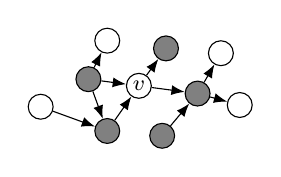
\begin{tikzpicture}[font={\footnotesize}, every node/.style={draw, inner sep=0 pt, minimum size=9 pt,
circle, fill=white}]
[font=\footnotesize, label distance=0 cm, inner sep=0.5 pt,
every node/.style={anchor=center},
]

\path
(0,0) node (a1) {}
-- ++(30:0.7) node[fill=gray] (a2) {}
-- ++(-70:0.7) node[fill=gray] (a3) {}
-- ++(55:0.7) node (a0) {\(v\)}
-- ++(125:0.7) node (a4) {}
(a3) ++(-5:0.7) node[fill=gray] (a5) {}
-- ++(50:0.7) node[fill=gray] (a6) {}
-- ++(125:0.7) node[fill=gray] (a7) {}
-- ++(-05:0.7) node (a8) {}
-- ++(-70:0.7) node (a9) {}
;

% DAG (Bayesian network)
\begin{scope}[-Latex]
\draw (a0) -- (a6) ;
\draw (a0) -- (a7) ;
\draw (a1) -- (a3);
\draw (a2) -- (a0) ;
\draw (a2) -- (a3) ;
\draw (a2) -- (a4) ;
\draw (a3) -- (a0) ;
\draw (a5) -- (a6) ;
\draw (a6) -- (a8) ;
\draw (a6) -- (a9) ;
\end{scope}

%% moralized DAG (Markov network)
%\begin{scope}[--]
%\draw (a0) -- (a6) ;
%\draw (a0) -- (a7) ;
%\draw (a1) -- (a3);
%\draw (a2) -- (a0) ;
%\draw (a2) -- (a3) ;
%\draw (a2) -- (a4) ;
%\draw (a3) -- (a0) ;
%\draw (a5) -- (a6) ;
%\draw (a6) -- (a8) ;
%\draw (a6) -- (a9) ;
%% extra edges
%\draw[dashed] (a1) -- (a2) ;
%\draw[dashed] (a0) -- (a5) ;
%\end{scope}

\end{tikzpicture}
\end{document}
